\documentclass[1p]{elsarticle_modified}
%\bibliographystyle{elsarticle-num}

%\usepackage[colorlinks]{hyperref}
%\usepackage{abbrmath_seonhwa} %\Abb, \Ascr, \Acal ,\Abf, \Afrak
\usepackage{amsfonts}
\usepackage{amssymb}
\usepackage{amsmath}
\usepackage{amsthm}
\usepackage{scalefnt}
\usepackage{amsbsy}
\usepackage{kotex}
\usepackage{caption}
\usepackage{subfig}
\usepackage{color}
\usepackage{graphicx}
\usepackage{xcolor} %% white, black, red, green, blue, cyan, magenta, yellow
\usepackage{float}
\usepackage{setspace}
\usepackage{hyperref}

\usepackage{tikz}
\usetikzlibrary{arrows}

\usepackage{multirow}
\usepackage{array} % fixed length table
\usepackage{hhline}

%%%%%%%%%%%%%%%%%%%%%
\makeatletter
\renewcommand*\env@matrix[1][\arraystretch]{%
	\edef\arraystretch{#1}%
	\hskip -\arraycolsep
	\let\@ifnextchar\new@ifnextchar
	\array{*\c@MaxMatrixCols c}}
\makeatother %https://tex.stackexchange.com/questions/14071/how-can-i-increase-the-line-spacing-in-a-matrix
%%%%%%%%%%%%%%%

\usepackage[normalem]{ulem}

\newcommand{\msout}[1]{\ifmmode\text{\sout{\ensuremath{#1}}}\else\sout{#1}\fi}
%SOURCE: \msout is \stkout macro in https://tex.stackexchange.com/questions/20609/strikeout-in-math-mode

\newcommand{\cancel}[1]{
	\ifmmode
	{\color{red}\msout{#1}}
	\else
	{\color{red}\sout{#1}}
	\fi
}

\newcommand{\add}[1]{
	{\color{blue}\uwave{#1}}
}

\newcommand{\replace}[2]{
	\ifmmode
	{\color{red}\msout{#1}}{\color{blue}\uwave{#2}}
	\else
	{\color{red}\sout{#1}}{\color{blue}\uwave{#2}}
	\fi
}

\newcommand{\Sol}{\mathcal{S}} %segment
\newcommand{\D}{D} %diagram
\newcommand{\A}{\mathcal{A}} %arc


%%%%%%%%%%%%%%%%%%%%%%%%%%%%%5 test

\def\sl{\operatorname{\textup{SL}}(2,\Cbb)}
\def\psl{\operatorname{\textup{PSL}}(2,\Cbb)}
\def\quan{\mkern 1mu \triangleright \mkern 1mu}

\theoremstyle{definition}
\newtheorem{thm}{Theorem}[section]
\newtheorem{prop}[thm]{Proposition}
\newtheorem{lem}[thm]{Lemma}
\newtheorem{ques}[thm]{Question}
\newtheorem{cor}[thm]{Corollary}
\newtheorem{defn}[thm]{Definition}
\newtheorem{exam}[thm]{Example}
\newtheorem{rmk}[thm]{Remark}
\newtheorem{alg}[thm]{Algorithm}

\newcommand{\I}{\sqrt{-1}}
\begin{document}

%\begin{frontmatter}
%
%\title{Boundary parabolic representations of knots up to 8 crossings}
%
%%% Group authors per affiliation:
%\author{Yunhi Cho} 
%\address{Department of Mathematics, University of Seoul, Seoul, Korea}
%\ead{yhcho@uos.ac.kr}
%
%
%\author{Seonhwa Kim} %\fnref{s_kim}}
%\address{Center for Geometry and Physics, Institute for Basic Science, Pohang, 37673, Korea}
%\ead{ryeona17@ibs.re.kr}
%
%\author{Hyuk Kim}
%\address{Department of Mathematical Sciences, Seoul National University, Seoul 08826, Korea}
%\ead{hyukkim@snu.ac.kr}
%
%\author{Seokbeom Yoon}
%\address{Department of Mathematical Sciences, Seoul National University, Seoul, 08826,  Korea}
%\ead{sbyoon15@snu.ac.kr}
%
%\begin{abstract}
%We find all boundary parabolic representation of knots up to 8 crossings.
%
%\end{abstract}
%\begin{keyword}
%    \MSC[2010] 57M25 
%\end{keyword}
%
%\end{frontmatter}

%\linenumbers
%\tableofcontents
%
\newcommand\colored[1]{\textcolor{white}{\rule[-0.35ex]{0.8em}{1.4ex}}\kern-0.8em\color{red} #1}%
%\newcommand\colored[1]{\textcolor{white}{ #1}\kern-2.17ex	\textcolor{white}{ #1}\kern-1.81ex	\textcolor{white}{ #1}\kern-2.15ex\color{red}#1	}

{\Large $\underline{10_{68}~(K10a_{67})}$}

\setlength{\tabcolsep}{10pt}
\renewcommand{\arraystretch}{1.6}
\vspace{1cm}\begin{tabular}{m{100pt}>{\centering\arraybackslash}m{274pt}}
\multirow{5}{120pt}{
	\centering
	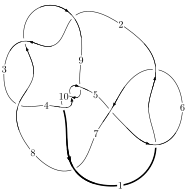
\includegraphics[width=112pt]{../../../GIT/diagram.site/Diagrams/png/152_10_68.png}\\
\ \ \ A knot diagram\footnotemark}&
\allowdisplaybreaks
\textbf{Linearized knot diagam} \\
\cline{2-2}
 &
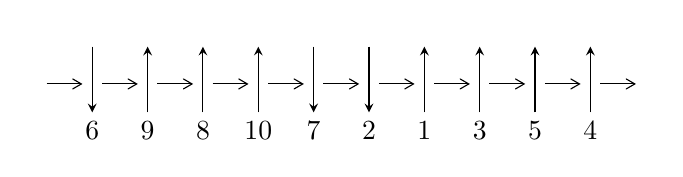
\begin{tikzpicture}[x=20pt, y=17pt]
	% nodes
	\node (C0) at (0, 0) {};
	\node (C1) at (1, 0) {};
	\node (C1U) at (1, +1) {};
	\node (C1D) at (1, -1) {6};

	\node (C2) at (2, 0) {};
	\node (C2U) at (2, +1) {};
	\node (C2D) at (2, -1) {9};

	\node (C3) at (3, 0) {};
	\node (C3U) at (3, +1) {};
	\node (C3D) at (3, -1) {8};

	\node (C4) at (4, 0) {};
	\node (C4U) at (4, +1) {};
	\node (C4D) at (4, -1) {10};

	\node (C5) at (5, 0) {};
	\node (C5U) at (5, +1) {};
	\node (C5D) at (5, -1) {7};

	\node (C6) at (6, 0) {};
	\node (C6U) at (6, +1) {};
	\node (C6D) at (6, -1) {2};

	\node (C7) at (7, 0) {};
	\node (C7U) at (7, +1) {};
	\node (C7D) at (7, -1) {1};

	\node (C8) at (8, 0) {};
	\node (C8U) at (8, +1) {};
	\node (C8D) at (8, -1) {3};

	\node (C9) at (9, 0) {};
	\node (C9U) at (9, +1) {};
	\node (C9D) at (9, -1) {5};

	\node (C10) at (10, 0) {};
	\node (C10U) at (10, +1) {};
	\node (C10D) at (10, -1) {4};
	\node (C11) at (11, 0) {};

	% arrows
	\draw[->,>={angle 60}]
	(C0) edge (C1) (C1) edge (C2) (C2) edge (C3) (C3) edge (C4) (C4) edge (C5) (C5) edge (C6) (C6) edge (C7) (C7) edge (C8) (C8) edge (C9) (C9) edge (C10) (C10) edge (C11) ;	\draw[->,>=stealth]
	(C1U) edge (C1D) (C2D) edge (C2U) (C3D) edge (C3U) (C4D) edge (C4U) (C5U) edge (C5D) (C6U) edge (C6D) (C7D) edge (C7U) (C8D) edge (C8U) (C9D) edge (C9U) (C10D) edge (C10U) ;
	\end{tikzpicture} \\
\hhline{~~} \\& 
\textbf{Solving Sequence} \\ \cline{2-2} 
 &
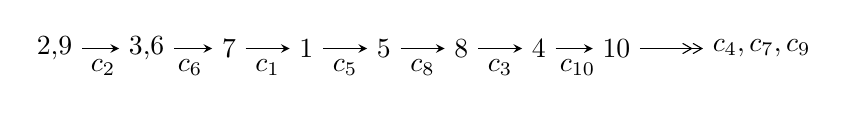
\begin{tikzpicture}[x=28pt, y=7pt]
	% node
	\node (A0) at (-1/8, 0) {2,9};
	\node (A1) at (17/16, 0) {3,6};
	\node (A2) at (17/8, 0) {7};
	\node (A3) at (25/8, 0) {1};
	\node (A4) at (33/8, 0) {5};
	\node (A5) at (41/8, 0) {8};
	\node (A6) at (49/8, 0) {4};
	\node (A7) at (57/8, 0) {10};
	\node (C1) at (1/2, -1) {$c_{2}$};
	\node (C2) at (13/8, -1) {$c_{6}$};
	\node (C3) at (21/8, -1) {$c_{1}$};
	\node (C4) at (29/8, -1) {$c_{5}$};
	\node (C5) at (37/8, -1) {$c_{8}$};
	\node (C6) at (45/8, -1) {$c_{3}$};
	\node (C7) at (53/8, -1) {$c_{10}$};
	\node (A8) at (9, 0) {$c_{4},c_{7},c_{9}$};

	% edge
	\draw[->,>=stealth]	
	(A0) edge (A1) (A1) edge (A2) (A2) edge (A3) (A3) edge (A4) (A4) edge (A5) (A5) edge (A6) (A6) edge (A7) ;
	\draw[->>,>={angle 60}]	
	(A7) edge (A8);
\end{tikzpicture} \\ 

\end{tabular} \\

\footnotetext{
The image of knot diagram is generated by the software ``\textbf{Draw programme}" developed by Andrew Bartholomew(\url{http://www.layer8.co.uk/maths/draw/index.htm\#Running-draw}), where we modified some parts for our purpose(\url{https://github.com/CATsTAILs/LinksPainter}).
}\phantom \\ \newline 
\centering \textbf{Ideals for irreducible components\footnotemark of $X_{\text{par}}$} 
 
\begin{align*}
I^u_{1}&=\langle 
- u^{11}+u^{10}-7 u^9+6 u^8-17 u^7+12 u^6-15 u^5+7 u^4-3 u^3- u^2+2 b-3 u+1,\\
\phantom{I^u_{1}}&\phantom{= \langle  }- u^{13}+u^{12}-10 u^{11}+9 u^{10}-36 u^9+30 u^8-54 u^7+43 u^6-22 u^5+20 u^4+10 u^3-2 u^2+4 a-3 u+3,\\
\phantom{I^u_{1}}&\phantom{= \langle  }u^{14}+9 u^{12}+u^{11}+31 u^{10}+6 u^9+48 u^8+11 u^7+27 u^6+2 u^5-2 u^4-8 u^3+u^2+1\rangle \\
I^u_{2}&=\langle 
4802 u^{17}-8268 u^{16}+\cdots+12107 b+16224,\;-1848 u^{17}-4160 u^{16}+\cdots+12107 a-35011,\\
\phantom{I^u_{2}}&\phantom{= \langle  }u^{18}- u^{17}+\cdots+6 u+1\rangle \\
I^u_{3}&=\langle 
- a u+2 b- a-2 u,\;a^2+a u+a+2 u,\;u^2+1\rangle \\
\\
\end{align*}
\raggedright * 3 irreducible components of $\dim_{\mathbb{C}}=0$, with total 36 representations.\\
\footnotetext{All coefficients of polynomials are rational numbers. But the coefficients are sometimes approximated in decimal forms when there is not enough margin.}
\newpage
\renewcommand{\arraystretch}{1}
\centering \section*{I. $I^u_{1}= \langle - u^{11}+u^{10}+\cdots+2 b+1,\;- u^{13}+u^{12}+\cdots+4 a+3,\;u^{14}+9 u^{12}+\cdots+u^2+1 \rangle$}
\flushleft \textbf{(i) Arc colorings}\\
\begin{tabular}{m{7pt} m{180pt} m{7pt} m{180pt} }
\flushright $a_{2}=$&$\begin{pmatrix}1\\0\end{pmatrix}$ \\
\flushright $a_{9}=$&$\begin{pmatrix}0\\u\end{pmatrix}$ \\
\flushright $a_{3}=$&$\begin{pmatrix}1\\- u^2\end{pmatrix}$ \\
\flushright $a_{6}=$&$\begin{pmatrix}\frac{1}{4} u^{13}-\frac{1}{4} u^{12}+\cdots+\frac{3}{4} u-\frac{3}{4}\\\frac{1}{2} u^{11}-\frac{1}{2} u^{10}+\cdots+\frac{3}{2} u-\frac{1}{2}\end{pmatrix}$ \\
\flushright $a_{7}=$&$\begin{pmatrix}\frac{1}{4} u^{13}-\frac{1}{4} u^{12}+\cdots-\frac{3}{4} u-\frac{1}{4}\\\frac{1}{2} u^{11}-\frac{1}{2} u^{10}+\cdots+\frac{3}{2} u-\frac{1}{2}\end{pmatrix}$ \\
\flushright $a_{1}=$&$\begin{pmatrix}u^3+2 u\\\frac{1}{4} u^{13}-\frac{1}{4} u^{12}+\cdots+\frac{5}{4} u-\frac{1}{4}\end{pmatrix}$ \\
\flushright $a_{5}=$&$\begin{pmatrix}-1\\-\frac{1}{4} u^{13}-\frac{1}{4} u^{12}+\cdots-\frac{1}{4} u-\frac{1}{4}\end{pmatrix}$ \\
\flushright $a_{8}=$&$\begin{pmatrix}- u\\u^3+u\end{pmatrix}$ \\
\flushright $a_{4}=$&$\begin{pmatrix}u^2+1\\- u^4-2 u^2\end{pmatrix}$ \\
\flushright $a_{10}=$&$\begin{pmatrix}u\\\frac{1}{4} u^{13}-\frac{1}{4} u^{12}+\cdots+\frac{5}{4} u-\frac{1}{4}\end{pmatrix}$\\&\end{tabular}
\flushleft \textbf{(ii) Obstruction class $= -1$}\\~\\
\flushleft \textbf{(iii) Cusp Shapes $= -2 u^{13}-17 u^{11}-3 u^{10}-55 u^9-20 u^8-79 u^7-46 u^6-39 u^5-33 u^4+9 u^3+9 u^2+7 u+3$}\\~\\
\newpage\renewcommand{\arraystretch}{1}
\flushleft \textbf{(iv) u-Polynomials at the component}\newline \\
\begin{tabular}{m{50pt}|m{274pt}}
Crossings & \hspace{64pt}u-Polynomials at each crossing \\
\hline $$\begin{aligned}c_{1},c_{6}\end{aligned}$$&$\begin{aligned}
&u^{14}-3 u^{13}+\cdots-7 u+2
\end{aligned}$\\
\hline $$\begin{aligned}c_{2},c_{3},c_{4}\\c_{8},c_{9},c_{10}\end{aligned}$$&$\begin{aligned}
&u^{14}+9 u^{12}+\cdots+u^2+1
\end{aligned}$\\
\hline $$\begin{aligned}c_{5}\end{aligned}$$&$\begin{aligned}
&u^{14}+7 u^{13}+\cdots+5 u+4
\end{aligned}$\\
\hline $$\begin{aligned}c_{7}\end{aligned}$$&$\begin{aligned}
&u^{14}-9 u^{13}+\cdots-115 u+26
\end{aligned}$\\
\hline
\end{tabular}\\~\\
\newpage\renewcommand{\arraystretch}{1}
\flushleft \textbf{(v) Riley Polynomials at the component}\newline \\
\begin{tabular}{m{50pt}|m{274pt}}
Crossings & \hspace{64pt}Riley Polynomials at each crossing \\
\hline $$\begin{aligned}c_{1},c_{6}\end{aligned}$$&$\begin{aligned}
&y^{14}-7 y^{13}+\cdots-5 y+4
\end{aligned}$\\
\hline $$\begin{aligned}c_{2},c_{3},c_{4}\\c_{8},c_{9},c_{10}\end{aligned}$$&$\begin{aligned}
&y^{14}+18 y^{13}+\cdots+2 y+1
\end{aligned}$\\
\hline $$\begin{aligned}c_{5}\end{aligned}$$&$\begin{aligned}
&y^{14}+y^{13}+\cdots+191 y+16
\end{aligned}$\\
\hline $$\begin{aligned}c_{7}\end{aligned}$$&$\begin{aligned}
&y^{14}+5 y^{13}+\cdots-69 y+676
\end{aligned}$\\
\hline
\end{tabular}\\~\\
\newpage\flushleft \textbf{(vi) Complex Volumes and Cusp Shapes}
$$\begin{array}{c|c|c}  
\text{Solutions to }I^u_{1}& \I (\text{vol} + \sqrt{-1}CS) & \text{Cusp shape}\\
 \hline 
\begin{aligned}
u &= -0.552436 + 0.381452 I \\
a &= \phantom{-}1.22078 - 1.57866 I \\
b &= \phantom{-}1.041840 + 0.481714 I\end{aligned}
 & -0.78724 - 4.41668 I & \phantom{-}3.49417 + 7.88625 I \\ \hline\begin{aligned}
u &= -0.552436 - 0.381452 I \\
a &= \phantom{-}1.22078 + 1.57866 I \\
b &= \phantom{-}1.041840 - 0.481714 I\end{aligned}
 & -0.78724 + 4.41668 I & \phantom{-}3.49417 - 7.88625 I \\ \hline\begin{aligned}
u &= -0.04509 + 1.43706 I \\
a &= \phantom{-}0.567049 - 0.433483 I \\
b &= \phantom{-}0.830389 + 0.784414 I\end{aligned}
 & -6.78342 - 2.90589 I & -2.10855 + 2.91897 I \\ \hline\begin{aligned}
u &= -0.04509 - 1.43706 I \\
a &= \phantom{-}0.567049 + 0.433483 I \\
b &= \phantom{-}0.830389 - 0.784414 I\end{aligned}
 & -6.78342 + 2.90589 I & -2.10855 - 2.91897 I \\ \hline\begin{aligned}
u &= \phantom{-}0.498731 + 0.157320 I \\
a &= -0.611249 - 0.332083 I \\
b &= \phantom{-}0.400528 + 0.482833 I\end{aligned}
 & \phantom{-}1.035520 + 0.368514 I & \phantom{-}9.33320 - 2.06000 I \\ \hline\begin{aligned}
u &= \phantom{-}0.498731 - 0.157320 I \\
a &= -0.611249 + 0.332083 I \\
b &= \phantom{-}0.400528 - 0.482833 I\end{aligned}
 & \phantom{-}1.035520 - 0.368514 I & \phantom{-}9.33320 + 2.06000 I \\ \hline\begin{aligned}
u &= -0.164790 + 0.466680 I \\
a &= -1.43454 + 0.30361 I \\
b &= -0.941064 + 0.407114 I\end{aligned}
 & -1.42730 + 1.54478 I & \phantom{-}1.163355 - 0.228482 I \\ \hline\begin{aligned}
u &= -0.164790 - 0.466680 I \\
a &= -1.43454 - 0.30361 I \\
b &= -0.941064 - 0.407114 I\end{aligned}
 & -1.42730 - 1.54478 I & \phantom{-}1.163355 + 0.228482 I \\ \hline\begin{aligned}
u &= -0.26550 + 1.53094 I \\
a &= -0.292054 - 0.268287 I \\
b &= \phantom{-}0.243278 - 0.917020 I\end{aligned}
 & -10.58650 - 6.18900 I & -1.00936 + 2.90508 I \\ \hline\begin{aligned}
u &= -0.26550 - 1.53094 I \\
a &= -0.292054 + 0.268287 I \\
b &= \phantom{-}0.243278 + 0.917020 I\end{aligned}
 & -10.58650 + 6.18900 I & -1.00936 - 2.90508 I\\
 \hline 
 \end{array}$$\newpage$$\begin{array}{c|c|c}  
\text{Solutions to }I^u_{1}& \I (\text{vol} + \sqrt{-1}CS) & \text{Cusp shape}\\
 \hline 
\begin{aligned}
u &= \phantom{-}0.33038 + 1.55103 I \\
a &= \phantom{-}1.76709 + 0.94504 I \\
b &= \phantom{-}1.211210 - 0.579083 I\end{aligned}
 & -13.5268 + 11.6370 I & -3.43423 - 6.31221 I \\ \hline\begin{aligned}
u &= \phantom{-}0.33038 - 1.55103 I \\
a &= \phantom{-}1.76709 - 0.94504 I \\
b &= \phantom{-}1.211210 + 0.579083 I\end{aligned}
 & -13.5268 - 11.6370 I & -3.43423 + 6.31221 I \\ \hline\begin{aligned}
u &= \phantom{-}0.19870 + 1.61232 I \\
a &= -1.71708 - 0.22802 I \\
b &= -1.286170 - 0.280982 I\end{aligned}
 & -15.6273 + 2.2414 I & -5.43859 - 0.46441 I \\ \hline\begin{aligned}
u &= \phantom{-}0.19870 - 1.61232 I \\
a &= -1.71708 + 0.22802 I \\
b &= -1.286170 + 0.280982 I\end{aligned}
 & -15.6273 - 2.2414 I & -5.43859 + 0.46441 I\\
 \hline 
 \end{array}$$\newpage\newpage\renewcommand{\arraystretch}{1}
\centering \section*{II. $I^u_{2}= \langle 4802 u^{17}-8268 u^{16}+\cdots+12107 b+16224,\;-1848 u^{17}-4160 u^{16}+\cdots+12107 a-35011,\;u^{18}- u^{17}+\cdots+6 u+1 \rangle$}
\flushleft \textbf{(i) Arc colorings}\\
\begin{tabular}{m{7pt} m{180pt} m{7pt} m{180pt} }
\flushright $a_{2}=$&$\begin{pmatrix}1\\0\end{pmatrix}$ \\
\flushright $a_{9}=$&$\begin{pmatrix}0\\u\end{pmatrix}$ \\
\flushright $a_{3}=$&$\begin{pmatrix}1\\- u^2\end{pmatrix}$ \\
\flushright $a_{6}=$&$\begin{pmatrix}0.152639 u^{17}+0.343603 u^{16}+\cdots+0.206988 u+2.89180\\-0.396630 u^{17}+0.682911 u^{16}+\cdots-1.61361 u-1.34005\end{pmatrix}$ \\
\flushright $a_{7}=$&$\begin{pmatrix}0.549269 u^{17}-0.339308 u^{16}+\cdots+1.82060 u+4.23185\\-0.396630 u^{17}+0.682911 u^{16}+\cdots-1.61361 u-1.34005\end{pmatrix}$ \\
\flushright $a_{1}=$&$\begin{pmatrix}0.987528 u^{17}-1.29215 u^{16}+\cdots+7.85430 u+5.72421\\-0.579830 u^{17}+0.616833 u^{16}+\cdots-4.42265 u-1.55001\end{pmatrix}$ \\
\flushright $a_{5}=$&$\begin{pmatrix}-1.52119 u^{17}+2.03023 u^{16}+\cdots-18.2674 u-3.39894\\0.275791 u^{17}-0.288263 u^{16}+\cdots+1.53308 u-0.490956\end{pmatrix}$ \\
\flushright $a_{8}=$&$\begin{pmatrix}- u\\u^3+u\end{pmatrix}$ \\
\flushright $a_{4}=$&$\begin{pmatrix}u^2+1\\- u^4-2 u^2\end{pmatrix}$ \\
\flushright $a_{10}=$&$\begin{pmatrix}1.50904 u^{17}-1.78484 u^{16}+\cdots+14.7282 u+7.52119\\-0.521516 u^{17}+0.492690 u^{16}+\cdots-4.87387 u-1.79698\end{pmatrix}$\\&\end{tabular}
\flushleft \textbf{(ii) Obstruction class $= -1$}\\~\\
\flushleft \textbf{(iii) Cusp Shapes $= \frac{31900}{12107} u^{17}-\frac{61944}{12107} u^{16}+\cdots+\frac{168364}{12107} u+\frac{112870}{12107}$}\\~\\
\newpage\renewcommand{\arraystretch}{1}
\flushleft \textbf{(iv) u-Polynomials at the component}\newline \\
\begin{tabular}{m{50pt}|m{274pt}}
Crossings & \hspace{64pt}u-Polynomials at each crossing \\
\hline $$\begin{aligned}c_{1},c_{6}\end{aligned}$$&$\begin{aligned}
&(u^9+u^8-2 u^7-3 u^6+u^5+3 u^4+2 u^3- u-1)^2
\end{aligned}$\\
\hline $$\begin{aligned}c_{2},c_{3},c_{4}\\c_{8},c_{9},c_{10}\end{aligned}$$&$\begin{aligned}
&u^{18}- u^{17}+\cdots+6 u+1
\end{aligned}$\\
\hline $$\begin{aligned}c_{5}\end{aligned}$$&$\begin{aligned}
&(u^9+5 u^8+12 u^7+15 u^6+9 u^5- u^4-4 u^3-2 u^2+u+1)^2
\end{aligned}$\\
\hline $$\begin{aligned}c_{7}\end{aligned}$$&$\begin{aligned}
&(u^9+3 u^8+8 u^7+13 u^6+17 u^5+17 u^4+12 u^3+6 u^2+u-1)^2
\end{aligned}$\\
\hline
\end{tabular}\\~\\
\newpage\renewcommand{\arraystretch}{1}
\flushleft \textbf{(v) Riley Polynomials at the component}\newline \\
\begin{tabular}{m{50pt}|m{274pt}}
Crossings & \hspace{64pt}Riley Polynomials at each crossing \\
\hline $$\begin{aligned}c_{1},c_{6}\end{aligned}$$&$\begin{aligned}
&(y^9-5 y^8+12 y^7-15 y^6+9 y^5+y^4-4 y^3+2 y^2+y-1)^2
\end{aligned}$\\
\hline $$\begin{aligned}c_{2},c_{3},c_{4}\\c_{8},c_{9},c_{10}\end{aligned}$$&$\begin{aligned}
&y^{18}+15 y^{17}+\cdots-16 y+1
\end{aligned}$\\
\hline $$\begin{aligned}c_{5}\end{aligned}$$&$\begin{aligned}
&(y^9- y^8+12 y^7-7 y^6+37 y^5+y^4-10 y^2+5 y-1)^2
\end{aligned}$\\
\hline $$\begin{aligned}c_{7}\end{aligned}$$&$\begin{aligned}
&(y^9+7 y^8+20 y^7+25 y^6+5 y^5-15 y^4+22 y^2+13 y-1)^2
\end{aligned}$\\
\hline
\end{tabular}\\~\\
\newpage\flushleft \textbf{(vi) Complex Volumes and Cusp Shapes}
$$\begin{array}{c|c|c}  
\text{Solutions to }I^u_{2}& \I (\text{vol} + \sqrt{-1}CS) & \text{Cusp shape}\\
 \hline 
\begin{aligned}
u &= \phantom{-}0.912264 + 0.491243 I \\
a &= -0.78567 - 1.24878 I \\
b &= -1.172470 + 0.500383 I\end{aligned}
 & -6.88799 + 7.08493 I & -1.57680 - 5.91335 I \\ \hline\begin{aligned}
u &= \phantom{-}0.912264 - 0.491243 I \\
a &= -0.78567 + 1.24878 I \\
b &= -1.172470 - 0.500383 I\end{aligned}
 & -6.88799 - 7.08493 I & -1.57680 + 5.91335 I \\ \hline\begin{aligned}
u &= \phantom{-}0.103396 + 1.069760 I \\
a &= -0.757195 - 0.604613 I \\
b &= -0.772920 + 0.510351 I\end{aligned}
 & -1.50643 + 2.09337 I & \phantom{-}4.51499 - 4.16283 I \\ \hline\begin{aligned}
u &= \phantom{-}0.103396 - 1.069760 I \\
a &= -0.757195 + 0.604613 I \\
b &= -0.772920 - 0.510351 I\end{aligned}
 & -1.50643 - 2.09337 I & \phantom{-}4.51499 + 4.16283 I \\ \hline\begin{aligned}
u &= \phantom{-}0.792965 + 0.741615 I \\
a &= \phantom{-}0.617829 - 0.014310 I \\
b &= \phantom{-}1.173910 + 0.391555 I\end{aligned}
 & -7.66122 - 1.33617 I & -3.28409 + 0.70175 I \\ \hline\begin{aligned}
u &= \phantom{-}0.792965 - 0.741615 I \\
a &= \phantom{-}0.617829 + 0.014310 I \\
b &= \phantom{-}1.173910 - 0.391555 I\end{aligned}
 & -7.66122 + 1.33617 I & -3.28409 - 0.70175 I \\ \hline\begin{aligned}
u &= -0.746849 + 0.515863 I \\
a &= \phantom{-}0.408531 - 0.597220 I \\
b &= -0.141484 + 0.739668 I\end{aligned}
 & -3.90681 - 2.45442 I & \phantom{-}1.67208 + 2.91298 I \\ \hline\begin{aligned}
u &= -0.746849 - 0.515863 I \\
a &= \phantom{-}0.408531 + 0.597220 I \\
b &= -0.141484 - 0.739668 I\end{aligned}
 & -3.90681 + 2.45442 I & \phantom{-}1.67208 - 2.91298 I \\ \hline\begin{aligned}
u &= -0.256179 + 1.094020 I \\
a &= \phantom{-}1.04650 - 1.39689 I \\
b &= \phantom{-}0.825933\phantom{ +0.000000I}\end{aligned}
 & -4.48831\phantom{ +0.000000I} & -4.65235 + 0. I\phantom{ +0.000000I} \\ \hline\begin{aligned}
u &= -0.256179 - 1.094020 I \\
a &= \phantom{-}1.04650 + 1.39689 I \\
b &= \phantom{-}0.825933\phantom{ +0.000000I}\end{aligned}
 & -4.48831\phantom{ +0.000000I} & -4.65235 + 0. I\phantom{ +0.000000I}\\
 \hline 
 \end{array}$$\newpage$$\begin{array}{c|c|c}  
\text{Solutions to }I^u_{2}& \I (\text{vol} + \sqrt{-1}CS) & \text{Cusp shape}\\
 \hline 
\begin{aligned}
u &= \phantom{-}0.118400 + 1.390980 I \\
a &= \phantom{-}0.194324 - 0.537825 I \\
b &= -0.141484 - 0.739668 I\end{aligned}
 & -3.90681 + 2.45442 I & \phantom{-}1.67208 - 2.91298 I \\ \hline\begin{aligned}
u &= \phantom{-}0.118400 - 1.390980 I \\
a &= \phantom{-}0.194324 + 0.537825 I \\
b &= -0.141484 + 0.739668 I\end{aligned}
 & -3.90681 - 2.45442 I & \phantom{-}1.67208 + 2.91298 I \\ \hline\begin{aligned}
u &= \phantom{-}0.00304 + 1.47476 I \\
a &= \phantom{-}2.29745 + 0.06492 I \\
b &= \phantom{-}1.173910 - 0.391555 I\end{aligned}
 & -7.66122 + 1.33617 I & -3.28409 - 0.70175 I \\ \hline\begin{aligned}
u &= \phantom{-}0.00304 - 1.47476 I \\
a &= \phantom{-}2.29745 - 0.06492 I \\
b &= \phantom{-}1.173910 + 0.391555 I\end{aligned}
 & -7.66122 - 1.33617 I & -3.28409 + 0.70175 I \\ \hline\begin{aligned}
u &= -0.18330 + 1.47754 I \\
a &= -2.21308 + 0.73195 I \\
b &= -1.172470 - 0.500383 I\end{aligned}
 & -6.88799 - 7.08493 I & -1.57680 + 5.91335 I \\ \hline\begin{aligned}
u &= -0.18330 - 1.47754 I \\
a &= -2.21308 - 0.73195 I \\
b &= -1.172470 + 0.500383 I\end{aligned}
 & -6.88799 + 7.08493 I & -1.57680 - 5.91335 I \\ \hline\begin{aligned}
u &= -0.243739 + 0.102909 I \\
a &= \phantom{-}3.19131 - 0.41254 I \\
b &= -0.772920 - 0.510351 I\end{aligned}
 & -1.50643 - 2.09337 I & \phantom{-}4.51499 + 4.16283 I \\ \hline\begin{aligned}
u &= -0.243739 - 0.102909 I \\
a &= \phantom{-}3.19131 + 0.41254 I \\
b &= -0.772920 + 0.510351 I\end{aligned}
 & -1.50643 + 2.09337 I & \phantom{-}4.51499 - 4.16283 I\\
 \hline 
 \end{array}$$\newpage\newpage\renewcommand{\arraystretch}{1}
\centering \section*{III. $I^u_{3}= \langle - a u+2 b- a-2 u,\;a^2+a u+a+2 u,\;u^2+1 \rangle$}
\flushleft \textbf{(i) Arc colorings}\\
\begin{tabular}{m{7pt} m{180pt} m{7pt} m{180pt} }
\flushright $a_{2}=$&$\begin{pmatrix}1\\0\end{pmatrix}$ \\
\flushright $a_{9}=$&$\begin{pmatrix}0\\u\end{pmatrix}$ \\
\flushright $a_{3}=$&$\begin{pmatrix}1\\1\end{pmatrix}$ \\
\flushright $a_{6}=$&$\begin{pmatrix}a\\\frac{1}{2} a u+\frac{1}{2} a+u\end{pmatrix}$ \\
\flushright $a_{7}=$&$\begin{pmatrix}-\frac{1}{2} a u+\frac{1}{2} a- u\\\frac{1}{2} a u+\frac{1}{2} a+u\end{pmatrix}$ \\
\flushright $a_{1}=$&$\begin{pmatrix}u\\-\frac{1}{2} a u+\frac{1}{2} a\end{pmatrix}$ \\
\flushright $a_{5}=$&$\begin{pmatrix}-1\\\frac{1}{2} a u+\frac{1}{2} a\end{pmatrix}$ \\
\flushright $a_{8}=$&$\begin{pmatrix}- u\\0\end{pmatrix}$ \\
\flushright $a_{4}=$&$\begin{pmatrix}0\\1\end{pmatrix}$ \\
\flushright $a_{10}=$&$\begin{pmatrix}u\\-\frac{1}{2} a u+\frac{1}{2} a+u\end{pmatrix}$\\&\end{tabular}
\flushleft \textbf{(ii) Obstruction class $= 1$}\\~\\
\flushleft \textbf{(iii) Cusp Shapes $= 2 a u-2 a-4$}\\~\\
\newpage\renewcommand{\arraystretch}{1}
\flushleft \textbf{(iv) u-Polynomials at the component}\newline \\
\begin{tabular}{m{50pt}|m{274pt}}
Crossings & \hspace{64pt}u-Polynomials at each crossing \\
\hline $$\begin{aligned}c_{1},c_{6},c_{7}\end{aligned}$$&$\begin{aligned}
&u^4- u^2+1
\end{aligned}$\\
\hline $$\begin{aligned}c_{2},c_{3},c_{4}\\c_{8},c_{9},c_{10}\end{aligned}$$&$\begin{aligned}
&(u^2+1)^2
\end{aligned}$\\
\hline $$\begin{aligned}c_{5}\end{aligned}$$&$\begin{aligned}
&(u^2- u+1)^2
\end{aligned}$\\
\hline
\end{tabular}\\~\\
\newpage\renewcommand{\arraystretch}{1}
\flushleft \textbf{(v) Riley Polynomials at the component}\newline \\
\begin{tabular}{m{50pt}|m{274pt}}
Crossings & \hspace{64pt}Riley Polynomials at each crossing \\
\hline $$\begin{aligned}c_{1},c_{6},c_{7}\end{aligned}$$&$\begin{aligned}
&(y^2- y+1)^2
\end{aligned}$\\
\hline $$\begin{aligned}c_{2},c_{3},c_{4}\\c_{8},c_{9},c_{10}\end{aligned}$$&$\begin{aligned}
&(y+1)^4
\end{aligned}$\\
\hline $$\begin{aligned}c_{5}\end{aligned}$$&$\begin{aligned}
&(y^2+y+1)^2
\end{aligned}$\\
\hline
\end{tabular}\\~\\
\newpage\flushleft \textbf{(vi) Complex Volumes and Cusp Shapes}
$$\begin{array}{c|c|c}  
\text{Solutions to }I^u_{3}& \I (\text{vol} + \sqrt{-1}CS) & \text{Cusp shape}\\
 \hline 
\begin{aligned}
u &= \phantom{-0.000000 -}1.000000 I \\
a &= \phantom{-}0.36603 - 1.36603 I \\
b &= \phantom{-}0.866025 + 0.500000 I\end{aligned}
 & -3.28987 - 2.02988 I & -2.00000 + 3.46410 I \\ \hline\begin{aligned}
u &= \phantom{-0.000000 -}1.000000 I \\
a &= -1.36603 + 0.36603 I \\
b &= -0.866025 + 0.500000 I\end{aligned}
 & -3.28987 + 2.02988 I & -2.00000 - 3.46410 I \\ \hline\begin{aligned}
u &= \phantom{-0.000000 } -1.000000 I \\
a &= \phantom{-}0.36603 + 1.36603 I \\
b &= \phantom{-}0.866025 - 0.500000 I\end{aligned}
 & -3.28987 + 2.02988 I & -2.00000 - 3.46410 I \\ \hline\begin{aligned}
u &= \phantom{-0.000000 } -1.000000 I \\
a &= -1.36603 - 0.36603 I \\
b &= -0.866025 - 0.500000 I\end{aligned}
 & -3.28987 - 2.02988 I & -2.00000 + 3.46410 I\\
 \hline 
 \end{array}$$\newpage
\newpage\renewcommand{\arraystretch}{1}
\centering \section*{ IV. u-Polynomials}
\begin{tabular}{m{50pt}|m{274pt}}
Crossings & \hspace{64pt}u-Polynomials at each crossing \\
\hline $$\begin{aligned}c_{1},c_{6}\end{aligned}$$&$\begin{aligned}
&(u^4- u^2+1)(u^9+u^8-2 u^7-3 u^6+u^5+3 u^4+2 u^3- u-1)^2\\
&\cdot(u^{14}-3 u^{13}+\cdots-7 u+2)
\end{aligned}$\\
\hline $$\begin{aligned}c_{2},c_{3},c_{4}\\c_{8},c_{9},c_{10}\end{aligned}$$&$\begin{aligned}
&((u^2+1)^2)(u^{14}+9 u^{12}+\cdots+u^2+1)(u^{18}- u^{17}+\cdots+6 u+1)
\end{aligned}$\\
\hline $$\begin{aligned}c_{5}\end{aligned}$$&$\begin{aligned}
&(u^2- u+1)^2\\
&\cdot(u^9+5 u^8+12 u^7+15 u^6+9 u^5- u^4-4 u^3-2 u^2+u+1)^2\\
&\cdot(u^{14}+7 u^{13}+\cdots+5 u+4)
\end{aligned}$\\
\hline $$\begin{aligned}c_{7}\end{aligned}$$&$\begin{aligned}
&(u^4- u^2+1)\\
&\cdot(u^9+3 u^8+8 u^7+13 u^6+17 u^5+17 u^4+12 u^3+6 u^2+u-1)^2\\
&\cdot(u^{14}-9 u^{13}+\cdots-115 u+26)
\end{aligned}$\\
\hline
\end{tabular}\newpage\renewcommand{\arraystretch}{1}
\centering \section*{ V. Riley Polynomials}
\begin{tabular}{m{50pt}|m{274pt}}
Crossings & \hspace{64pt}Riley Polynomials at each crossing \\
\hline $$\begin{aligned}c_{1},c_{6}\end{aligned}$$&$\begin{aligned}
&(y^2- y+1)^2\\
&\cdot(y^9-5 y^8+12 y^7-15 y^6+9 y^5+y^4-4 y^3+2 y^2+y-1)^2\\
&\cdot(y^{14}-7 y^{13}+\cdots-5 y+4)
\end{aligned}$\\
\hline $$\begin{aligned}c_{2},c_{3},c_{4}\\c_{8},c_{9},c_{10}\end{aligned}$$&$\begin{aligned}
&((y+1)^4)(y^{14}+18 y^{13}+\cdots+2 y+1)(y^{18}+15 y^{17}+\cdots-16 y+1)
\end{aligned}$\\
\hline $$\begin{aligned}c_{5}\end{aligned}$$&$\begin{aligned}
&(y^2+y+1)^2(y^9- y^8+12 y^7-7 y^6+37 y^5+y^4-10 y^2+5 y-1)^2\\
&\cdot(y^{14}+y^{13}+\cdots+191 y+16)
\end{aligned}$\\
\hline $$\begin{aligned}c_{7}\end{aligned}$$&$\begin{aligned}
&(y^2- y+1)^2\\
&\cdot(y^9+7 y^8+20 y^7+25 y^6+5 y^5-15 y^4+22 y^2+13 y-1)^2\\
&\cdot(y^{14}+5 y^{13}+\cdots-69 y+676)
\end{aligned}$\\
\hline
\end{tabular}
\vskip 2pc
\end{document}